\scanpage{134}\mspage{8}
% archive sheet number: 133 (upper left)
Mais on veut une factorisation de $f$, flèche quelconque dans $M$ en
\[
f=pi,\quad\text{avec }p\in C_{0*}\quad\uuline{\text{et}}\quad i\in\widetilde C_0,
\]
donc il faut encore \unsure{énoncer} une propriété, assurant que les $i_\alpha(f)$ sont dans $\unsure{\widetilde C_0|\widetilde C}$. On aura $\unsure{\simeq|=}$ quelque \unsure{chose} de plus précis. Introduisons donc
\[
\begin{aligned}
C'_0={}&\text{plus petit sous-ensemble de }\mathrm{Fl}\,M\\
&\text{contenant }C_0,\text{ stable par cochangement de}\ \deleted{\unsure{petites}}\\
&\text{base (chaque fois qu'il existe),}\ \deleted{\unsure{et par}}
\end{aligned}\tag*{1.18.}
\]
\[
\begin{aligned}
C''_0={}&\deleted{\text{\unsure{ensemble des sommes amalgamées de flèches}}}\ \inserted{\text{\unsure{flèches qui sont soit}}}\\
&\text{dans }C'_0,\text{ soit des sommes amalgamées}\\
&\inserted{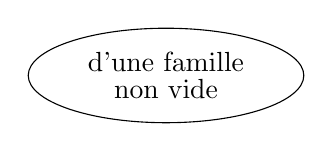
\begin{tikzpicture}[baseline=(t.base)]
\node[inner sep=2pt] (t) {\shortstack{d'une famille\\non \uuline{vide}}};
\draw (t.center) ellipse (1.75cm and .6cm);
\end{tikzpicture}}\quad\text{\unsure{telles flèches}}\ \deleted{\text{\unsure{de flèches}}}\quad A\xrightarrow{i_\alpha}B_\alpha\\
&\text{de }\unsure{\simeq|=}\text{ source }\inserted{A},\quad i_\alpha\in C'_0;\text{ la flèche}\\
&A\longrightarrow B=\coprod_{\alpha\,(A)}B_\alpha\quad\text{est dans }C'_0.
\end{aligned}
\]
% slanted; crossed block in the left margin
\margin{\deleted{\deleted{\unsure{Variante|Voir note|Vérifier}} \uline{NB} \unsure{Il n'est pas sûr que} les $i\in C''_0$ soient \unsure{quarrables}, si les \unsure{changements} de base \illegible{4} \unsure{Remarqué d'ici}.}}

(La condition 1.16. implique que les éléments de $C'_0$ sont \unsure{coquarrables}, et cela suffit, avec la condition de stabilité de $M$ par \deleted{\unsure{petites}} $\varinjlim$ filtrantes, à assurer que les sommes amalgamées infinies envisagées \deleted{\unsure{sont bien}} existent dans $M$.)
\[
\begin{aligned}
C'''_0={}&\text{plus petit sous-ensemble de }\mathrm{Fl}\,M\\
&\text{contenant }C''_0,\text{ et stable de plus}\\
&\text{par limites inductives ordinales}\\
&\text{strictes, i.e. pour un système}\\
&\text{inductif ordinal }(A_\alpha)_{\alpha<\alpha_0},\\
&\text{tel que pour }\alpha\text{ ordinal limite}\\
&\text{on ait } A_\alpha\unsure{\Leftarrow|\leftarrow}\varinjlim_{\alpha'\in I_\alpha}A_{\alpha'},\text{ si}\\
&\text{les morphismes de transition}\\
&i_{\beta,\alpha}:A_\alpha\longrightarrow A_\beta\quad\text{sont dans }C''_0,\\
&\text{\unsure{les|de}}\quad\unsure{\equiv|=}\quad\text{les morphismes canoniques}\\
&A_\alpha\xrightarrow{i_\alpha}\varinjlim_{\beta\in I_{\alpha_0}}A_\beta
\end{aligned}\tag*{1.19.}
\]
\margin{$C_0\subset C'_0\subset C''_0\subset C'''_0$}
\margin{\uline{NB} $C''_0$ est \deleted{\uuline{\unsure{déjà|d'après}} \unsure{au plus}} \deleted{\unsure{petit que le}} plus petit ens. de flèches contenant $C_0$ et stable par \unsure{cochgt} de base et par petites sommes amalgamées}
